% Author: Zhenyun Xie

\chapter{Theoretical and Programming Methodologies of Photonic Integrated Circuits} \label{chap:fundamentals}
The rapid advancement of silicon photonics has transitioned integrated optical systems from application-specific, static designs toward versatile, software-defined architectures.
This shift enables the dynamic manipulation of light, allowing a single hardware platform to support reconfigure networking functions and connections.
This chapter introduces the theoretical foundations and programming methodologies required to understand and control programmable PICs.
It begins with the fundamental building blocks, including 50:50 splitters, waveguide crossings, phase shifters, and 2x2 programmable unit cells (PUCs).
The transfer-matrix models of these components are presented to describe how optical signals are manipulated within the circuit.
The discussion then extends to circuit topologies constructed from these unit cells, including feedforward mesh architectures and recirculating mesh architectures.
Building on these physical structures, a graph-theoretic abstraction is developed to model photonic circuits as nodes and edges, enabling automated routing and configuration synthesis.
Finally, the chapter introduces the principles of Software-Defined Networking (SDN) to establish a control layer that connects low-level photonic hardware with higher-level network management.

\section{Basic building blocks} \label{sec:functional_blocks} % (fold)
\subsection{50:50 splitter} \label{sub:splitter} % (fold)
The 50:50 splitter, or 3dB coupler, serves as the foundational element for signal distribution and interferometric modulation within photonic integrated circuits, functioning primarily through two distinct physical mechanisms: evanescent coupling and self-imaging.
% DCs
Directional Couplers (DCs) serve as passive splitting elements by placing two waveguides in extreme proximity, typically separated by a gap of only a few hundred nanometers.
This arrangement facilitates evanescent coupling, a physical phenomenon where light tunnels between adjacent cores as their electromagnetic fields overlap.
While DCs are valued for their exceptionally low insertion loss (typically ranging from 0.1 to 0.5 dB) and their ability to be dynamically tuned via phase shifters for precise amplitude control, they are inherently sensitive to environmental and manufacturing conditions.
Because the power-splitting ratio is a strict function of the coupling length and waveguide separation, even nanometric deviations during fabrication or shifts in the operating wavelength can result in significant power imbalances.
Consequently, while DCs offer high performance, their delicate nature makes them susceptible to yield issues in large-scale systems.

%MMI
In contrast, Multimode Interferometers (MMIs) offer a more resilient alternative for routing and splitting optical signals by exploiting the self-imaging effect.
When an optical field enters a widened multimode waveguide region, it excites multiple propagation modes that interfere constructively at specific periodic intervals, forming replicas of the input signal at the output ports.
Although MMIs generally has slightly higher insertion losses (approximately 0.2 to 0.8 dB) than directional couplers, they provide superior fabrication tolerance and structural robustness.
Their performance is less dependent on ultra-precise waveguide gaps, ensuring high reliability and functional yield in high-density photonic chips.
Furthermore, MMIs are favored for their broadband specs, maintaining stable 50:50 splitting ratios across a wide spectral range, which is critical for wavelength-division multiplexing (WDM) applications.

Regardless of the chosen architecture, real-world imperfections, such as surface roughness and lithographic variations, inevitably lead to splitting imbalances and unintended phase shifts.
In a switch matrix, a deviation from the ideal 50:50 ratio—even by a few percent—limits the maximum achievable extinction ratio of subsequent Mach-Zehnder Interferometers (MZIs).
For the large-scale integrated circuits presented in later chapters, the MMI was selected as the primary building block due to its ability to maintain high performance and yield despite the environmental and manufacturing fluctuations inherent in mass-produced silicon photonics.

\subsection{Phase shifter} \label{sub:phase_shifter} % (fold)
The phase shifter is the essential active component in programmable photonic integrated circuits, responsible for modulating the phase of the optical field within a waveguide.
By inducing a controllable phase shift, these devices enable the constructive or destructive interference required for switching, routing, and signal processing.
Mathematically, the accumulated optical phase $\phi$ along a waveguide of length $L$ is given by:
\begin{equation}
    \phi = \frac{2 \pi n_{\mathrm{eff}} L}{\lambda}
\end{equation}
where $n_{\mathrm{eff}}$ denotes the effective refractive index of the guided mode and $\lambda$ is the free-space optical wavelength.
A variation in either $n_{\mathrm{eff}}$ or $L$ produces a corresponding change in the optical phase, which forms the basis of phase-shifting devices.
In silicon photonics, integrated phase shifting is primarily achieved through either electro-optic PS (EOPS) either thermos-optic PS (TOPS).
While electro-optic shifters based on plasma dispersion offer high-speed modulation in the nanoseconds timescales, they often suffer from relatively high insertion losses due to carrier absorption and require complex manufacturing processing.
In contrast, thermo-optic phase shifters exploit silicon's high thermo-optic coefficient to modify the refractive index locally through heat.
Although slower than electro-optic effects, thermal shifters are simpler to implement, and exhibit negligible insertion loss, making them the preferred choice for the high-density circuit.
Design evolution has focused on enhancing thermal efficiency as actuator density increases.

% TOPS performance
The TOPS is mainly determined by two key parameters: the half-wave power (Pπ), which indicates the electrical power required to produce a π phase shift,
and the reconfiguration speed, typically defined by the 10-90\% rise and fall times of the optical response.
Figure~\ref{fig:ch2-ps} illustrates schematic of three different structure of thermo-optic phase shifter.
Conventional metal heaters on oxide cladding suffer from heat leakage into the substrate, resulting in high Pπ and thermal crosstalk.
Vertical trench structures improve lateral thermal confinement, lowering power consumption and enabling tighter actuator spacing.
For maximum efficiency, suspended silicon structures remove the underlying substrate to achieve near-complete thermal isolation, minimizing power usage and crosstalk.
\begin{figure}[h]
    \begin{center}
        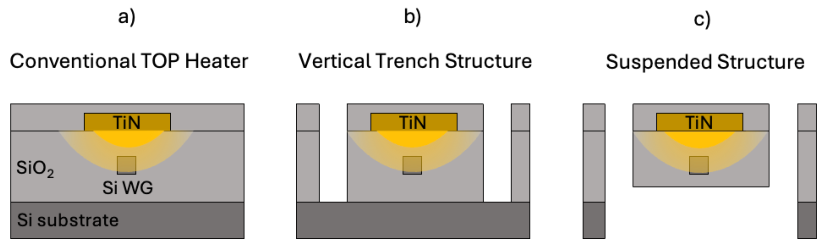
\includegraphics{figures/ch2-ps.pdf}
    \end{center}
    \caption{Cross-sectional schematic of a thermo-optic phase shifter employing a TiN (titanium nitride) heater.
        (a) Conventional phase shifter (b) Vertical trenched (c) Full suspended
    }\label{fig:ch2-ps}
\end{figure}

\subsection{2x2 programmable unit cells}\label{sub:pucs} % (fold)
The 2x2 Mach-Zehnder Interferometer (MZI) serves as the physical implementation of the Programmable Unit Cell (PUC), which is defined in this thesis as the fundamental building block of the system.
Figure~\ref{fig:ch2-puc} structurally demonstrate a PUC, a integrated puc is composed of a symmetric four-port configuration consisting of an initial 50:50 input splitter, two independent waveguide interference arms of length $L$, at least one active phase shifter integrated into these arms, and a final 50:50 output coupler that recombines the optical fields.
The operational physics of the device relies on the principle of dual-beam interference, where an incoming optical signal is first divided into two coherent components by the input splitter (MMI or DC),
As these two signals propagate through the interference arms, their relative phase relationship is dynamically adjusted via thermo-optic or electro-optic phase shifters, which modify the effective refractive index ($n_{\mathrm{eff}}$) of the waveguide mode to accumulate a specific optical phase $\phi = 2\pi n_{\mathrm{eff}} L / \lambda$.
Upon reaching the output coupler, the two optical signals interfere constructively or destructively depending on their accumulated phase difference.
This interference enables the device to control the power distribution between the output ports, allowing it to function as either a tunable coupler or an optical switch.
Figure~\ref{fig:ch2-puc}(c) illustrates three operating states of the PUC: cross, bar, and tunable.
\begin{figure}[h]
    \begin{center}
        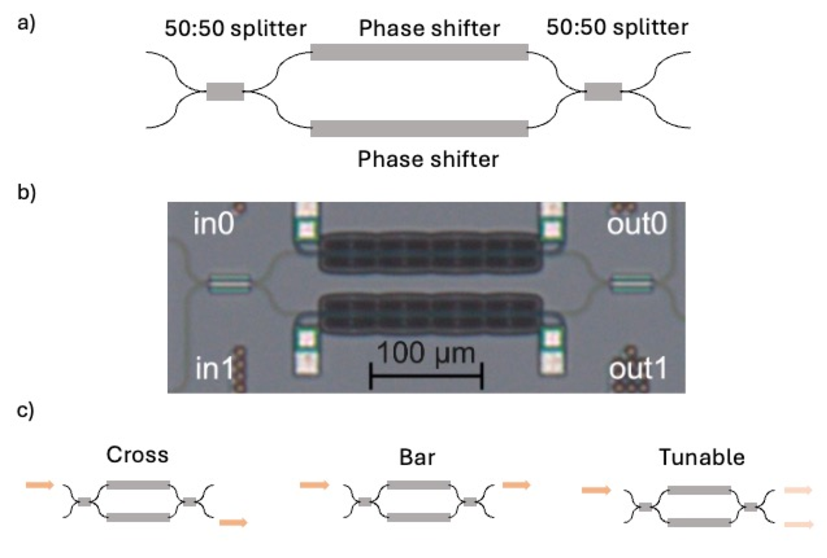
\includegraphics{figures/ch2-puc.pdf}
    \end{center}
    \caption{Structure and Operation of the 2x2 PUC
        (a) Schematic of the 2x2 PUC consisting of two 50:50 splitters and two phase shifters. (b) Optical micrograph of the fabricated element.
        (c) Operating states of the device, demonstrating cross, bar, and tunable transmission configurations.
    }\label{fig:ch2-puc}
\end{figure}
For an ideal PUC, the scattering matrix incorporates the effects of propagation losses and the inherent $\pi/2$ phase shift introduced by the 3-dB couplers, which is mathematically represented by the imaginary unit $-j$.
According to the device matrix under ideal lossless conditions, the overall scattering matrix can be expressed in two primary forms depending on the placement of additional phase shifters:
\begin{equation}
    \label{eq:ch2-puc}
    \begin{aligned}
        S = -j e^{j\Delta}
        \begin{pmatrix}
            \sin\theta & \cos\theta  \\
            \cos\theta & -\sin\theta
        \end{pmatrix}
    \end{aligned}
\end{equation}
In equation~\eqref{eq:ch2-puc}, $\theta$ denotes the interference phase, which is determined by the differential phase shift between the two heaters and is calculated as $\theta = (\phi_{up} - \phi_{lo})/2$.
For an ideal PUC, the differential phase shift $\theta$ equals zero, indicating that the passive state of the PUC corresponds to the cross state.
The term $\Delta$ represents the common phase shift, a common drive in both heaters providing a global phase offset that leads to independent control of the device phase without affecting the power ratio, and is calculated as $\Delta = (\phi_{up} + \phi_{lo})/2$.

The PUC prominence in large-scale integrated systems stems from its scalability and compatibility with high-yield manufacturing using robust components.
However, when circuits scale to thousands of PUCs, nanometric fabrication deviations in the two arms can induce imbalances, resulting in residual optical power leaking into unintended ports and accumulating across cascaded stages.
This phenomenon is detailed in Chapter~\ref{chap:ocs_archs}.

\subsection{Crossing}\label{sub:crossing} % (fold)
In the large-scale, high density PICs, besides PUCs serving as the fundamental switching units, a vast number of waveguide crossings are required for routing.
These components are not only passive interconnects; they constitute a critical bottleneck in system design.
Without careful optimization, the cumulative effects of hundreds of crossings can severely limit the overall optical bandwidth, introduce significant insertion loss, and generate detrimental optical crosstalk, thereby reducing the signal-to-noise ratio (SNR) of the entire chip.

Several classes of waveguide crossings have been explored to balance footprint, loss, and crosstalk.
MMI-based crossings exploit the self-imaging effect, where an optical field entering a widened multimode region excites multiple propagation modes that interfere constructively at specific periodic intervals to form replicas of the input signal.
By concentrating the optical power at the center of the intersection, this mechanism significantly reduces diffractive leakage into transverse arms and offers superior fabrication tolerance and structural robustness compared.
In parallel, sub-wavelength gratings (SWG) crossings employ metamaterial engineering through periodically segmented waveguides to artificially tune the effective refractive index, allowing the optical mode to expand adiabatically and cross the intersection with suppressed scattering.
Furthermore, taper-based crossings utilize parabolic or elliptical geometries to increase the mode size before reaching the intersection, thereby reducing the divergence angle and ensuring the optical field is recaptured by the receiving waveguide with minimal loss or crosstalk.

\section{Photonics mesh architectures}\label{sec:mesh_architectures}
By leveraging the interconnectivity of the fundamental building blocks detailed in section \ref{sec:functional_blocks}, a wide variety of photonic mesh architectures can be synthesized to achieve complex and high-dimensional optical functions.
These topologies are primarily categorized based on their signal flow characteristics into two classes: feedforward meshes, which maintain a unidirectional light path for linear transformations and switching, and recirculating (or circular) meshes, which incorporate feedback loops to enable resource reuse and spectral filtering.
This section explores the structural properties, scaling laws, and operational principles of these mesh geometries, which form the physical foundation of software-defined photonic systems.

\subsection{Feedforward mesh}\label{sub:feedforward} % (fold)
Feedforward meshes are characterized by an acyclic graph structure where optical signals propagate in a strictly unidirectional manner from input to output ports.
By eliminating feedback loops, these architectures ensure predictable latency and simplified phase control, making them the workhorse of both programmable computing and high-speed switching.
While architectures like the Reck and Clements designs have gained significant traction in photonic computing for performing unitary matrix multiplications in optical neural networks,
this thesis primarily focuses on the application of feedforward meshes within data center networks.

In this context, the mesh serves as a high-capacity, transparent switching fabric capable of routing massive data streams with minimal power consumption.
The selection of a specific topology involves a delicate balancing act between connectivity and physical constraints.
Common architectures include Benes, Path-Independent Loss (PILOSS), Banyan, etc.
Despite their advantages, scaling feedforward meshes to the port counts required by modern datacenters introduces bottlenecks.
Hardware complexity grows rapidly, leading to large chip footprints and increased fabrication risks.
Furthermore, optical performance is often limited by the accumulation of insertion loss and coherent crosstalk from hundreds of waveguide crossings and splitters, which can severely limit the SNR and lead to internal blocking under certain traffic patterns.
A rigorous evaluation of these trade-offs and the optimization of these switching fabrics for large-scale deployment will be discussed in detail in Chapter \ref{chap:ocs_archs}.
\subsection{Recirculating mesh}\label{sub:circular} % (fold)
Recirculating meshes, represent a paradigm shift from application-specific designs toward general-purpose photonic processors.
Unlike feedforward architectures where light follows a fixed, unidirectional path, recirculating meshes allow for the creation of feedback loops and multi-directional routing.
By interconnecting PUCs in a closed-loop grid, the hardware becomes a flexible platform where various optical functions can be software-defined without changing the physical chip layout.

The defining characteristic of these meshes is their ability to synthesize a wide array of optical circuits on-demand.
By dynamically configuring each PUC into one of three primary states—bar, cross, or tunable (see Fig~\ref{fig:ch2-puc}(c))—the user can effectively configure specific sub-circuits within the physical hardware, such as recursive filters (FIR/IIR) and tunable delay lines.
While these meshes are theoretically universal and capable of emulating any feedforward topology, doing so requires a higher density of PUCs to manage the internal routing necessary to mimic unidirectional flow.

As illustrated in figure\ref{fig:ch2-recirculating_topologies}, various grid geometries have been explored, including square, triangular, and hexagonal layouts.
Among these, the hexagonal architecture is widely regarded as the superior choice for high-density integration due to its unique topological advantages.
One of the primary benefits of the hexagonal arrangement is its higher spatial utilization and connectivity per unit area, which allows for a more compact and efficient footprint.
Furthermore, the hexagonal architecture supports greater routing flexibility and increased degrees of freedom for programming, enabling the synthesis of more complex functions with reduced hardware overhead.
\begin{figure}[h]
    \begin{center}
        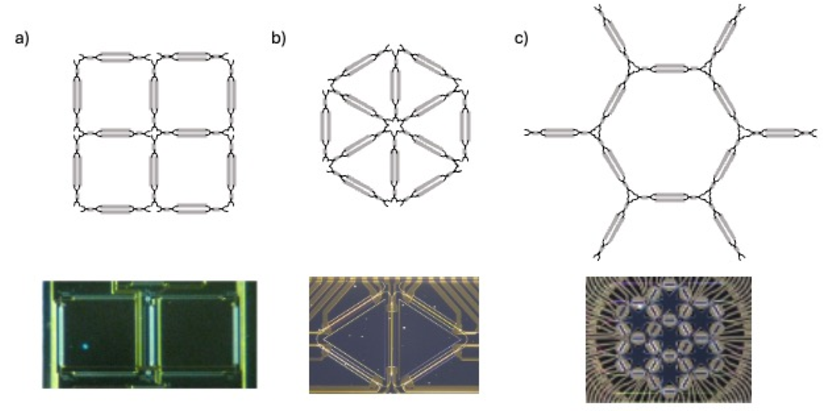
\includegraphics{figures/ch2-recir-mesh.pdf}
    \end{center}
    \caption{Recirculating integrated circuit mesh arrangements. The schematic representation (top) and microscope photography (bottom)
        (a) Square mesh, (b) Triangular mesh, and (c) Hexagonal mesh
    }\label{fig:ch2-recirculating_topologies}
\end{figure}
\subsubsection{Hexagonal mesh}\label{sub:hexagonal} % (fold)
The general-purpose photonic processor in this work consists of a hexagonal arrangement of 72 PUCs and 28 optical ports connected to photodetectors.
The schematic of the core is shown in Figure\ref{fig:ch2-smartlight}. It should be noted that bottom ports cannot be used as optical I/O;
they are not directly connected to photodetectors in the hardware design.
\begin{figure}[h]
    \begin{center}
        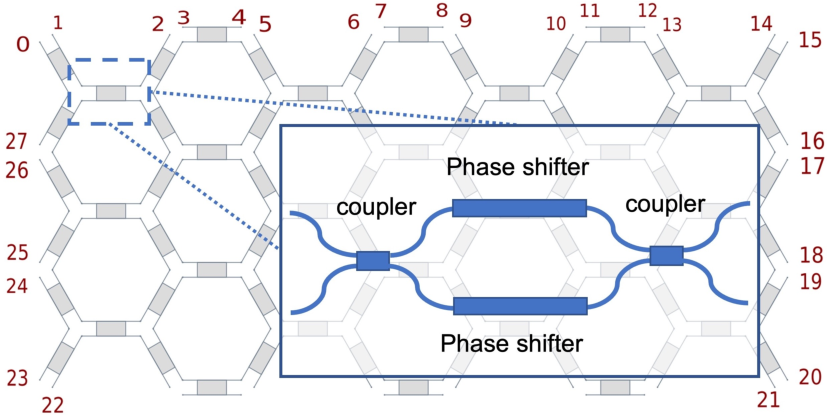
\includegraphics{figures/ch2-smartlight.pdf}
    \end{center}
    \caption{Schematic representation of the programmable processor core based on hexagonal cells.
    }\label{fig:ch2-smartlight}
\end{figure}

\section{Graph-Theoretic Modeling of Photonic Circuits}\label{sec:graph}
Despite the potential of the aforementioned circuits, large-scale meshes introduce significant control challenges.
The conventional configuration of these circuits relies on sequential tuning, where each individual PUC is set one by one to achieve the target behavior.
This manual approach is not only labor-intensive and error-prone but also fails to scale as the number of PUCs reaches the hundreds or thousands.

To this end, a truly software-defined processor necessitates a shift in how we represent and manipulate the underlying hardware.
A graph-theoretic abstraction is proposed, providing a mathematical approach that translates the physical topology into a logical map of nodes and edges.
By representing the circuit as a graph G=(V,E), where V is a set of vertices (nodes) and E is a set of edges, we can leverage mature network algorithms to automate routing, optimize performance, and synthesize complex optical functions through software commands.
The flexibility of the graph model allows for different levels of abstraction depending on the circuit topology and the specific application requirements.
One challenge in graph representation of hexagonal mesh is the feedback loops in the circuit.
To address this, we chose the directed graph with eight artificial nodes for our model, where each port of a PUC is represented with two artificial nodes, for inbound and outbound of the signal.
The PUC phase shifters are modeled by arcs with the direction of input and output ports.
Figure\ref{fig:ch2-hexagonal-graph} shows the graph representing the hexagonal mesh fig\ref{fig:ch2-smartlight}.
\begin{figure}[h]
    \begin{center}
        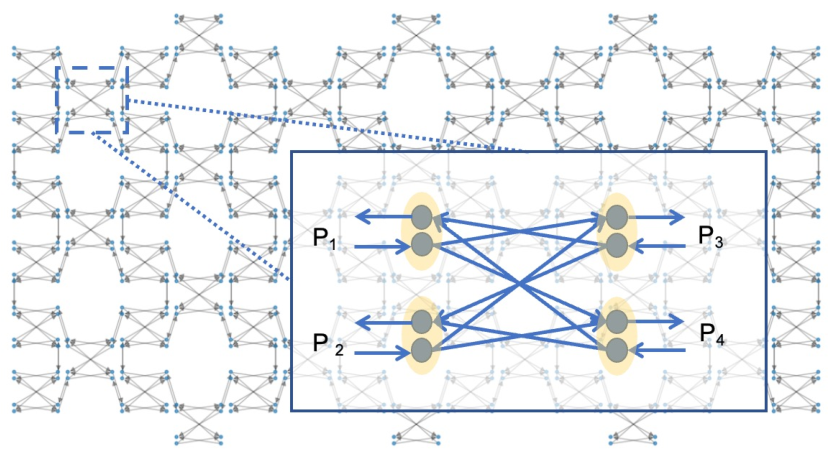
\includegraphics{figures/ch2-hexagonal-graph.pdf}
    \end{center}
    \caption{Graph-based representation of the photonic mesh. The inset depicts a detailed representation of the edges and vertices in a PUC.
    }\label{fig:ch2-hexagonal-graph}
\end{figure}

The graph representation incorporates performance metrics for each connection, which means each arc is assigned a weight as expressed by the following equation~\eqref{eq:ch2-graph_weight}:
\begin{equation}
    w = c_1 \cdot \textit{IL} + c_2 \cdot \textit{BUL} + c_3 \cdot P + \dots
    \label{eq:ch2-graph_weight}
\end{equation}
where IL is the PUC insertion loss, BUL is the PUC basic uni length, and $P_c$ is the PUC power consumption.
Hence the weight can be calculated according to these figures of merit (FoMs) by only changing the distribution of weights {$c_i$}
The graph-based mesh can be systematically connected in a predetermined manner, thus enabling symmetrical hexagonal photonic meshes of different sizes to be simulated.

Conversely, for feedforward architectures (such as Benes or PILOSS meshes), the abstraction can be significantly simplified.
Since the signal flow is strictly unidirectional and acyclic, a single node can often represent an entire PUC or a specific junction.
As illustrated in Figure\ref{fig:ch2-benes-graph}, the benes mesh can be abstracted at different levels of granularity depending on the computational requirements.
In the PUC-level graph (Fig\ref{fig:ch2-benes-graph}(a)), each node represents an entire 2x2 PUC.
This simplified representation is highly efficient for high-level operations, such as calculating total hardware complexity or performing rapid path routing across large-scale meshes, as the reduced number of nodes minimizes the search space for pathfinding algorithms.

In contrast, the port-level graph (Fig\ref{fig:ch2-benes-graph}(b)) provides a higher-resolution abstraction where each node corresponds to an individual optical port of a PUC.
While this increases the total number of nodes and consequently slows down the routing speed in massive meshes, it offers significantly more operational detail.
This level of abstraction allows the control software not only to find a valid path but also to automatically derive the specific configuration (bar, cross, or tunable) for every PUC along that path.
Furthermore, as indicated by the yellow nodes in figures, this model explicitly accounts for waveguide crossings, which are critical bottlenecks for optical performance.
\begin{figure}[h]
    \begin{center}
        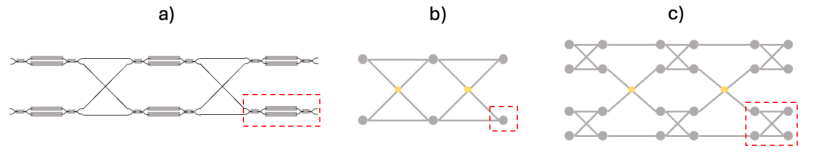
\includegraphics{figures/ch2-benes-graph.pdf}
    \end{center}
    \caption{Graph-based representation of the photonic mesh. The inset depicts a detailed representation of the edges and vertices in a PUC.
    }\label{fig:ch2-benes-graph}
\end{figure}
Just as with the hexagonal recirculating meshes, the edges in these feedforward graphs can be assigned weights based on specific FoMs.

\section{Software-Defined Network (SDN)}\label{sec:sdn}

